\section{experiments}

	4 big experiments have been executed.
	
	\begin{itemize}
		\item noise analysis
		\item tracking, manually changing the set points
		\item tracking using sine/stair functions
		\item disturbances
	\end{itemize}

\subsection{Simulink}
Figure~\ref{fig:simulink measurement diagram} contains the Simulink diagram used for the measurements. The same estimator subsystem as in the previous section was used. With a cut-off frequency of $f_c=2Hz$, the saturation block is not necessary here. As Simulink itself will limit the output to the motor.
	\begin{figure}[H]
	\centering
	\begin{subfigure}[b]{0.55\textwidth}
		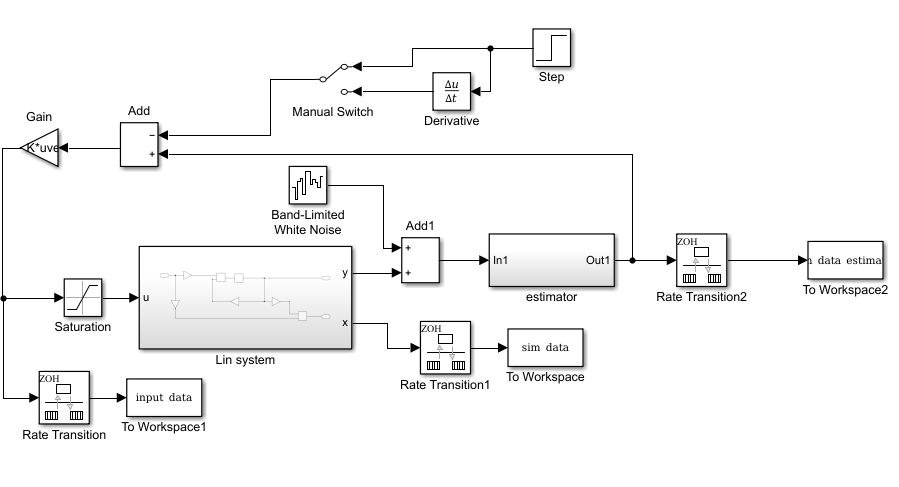
\includegraphics[width=\textwidth]{./part4_experiments/not_generated/simulink_main.png}
		\caption{main diagram}
	\end{subfigure}
	\begin{subfigure}[b]{0.45\textwidth}
		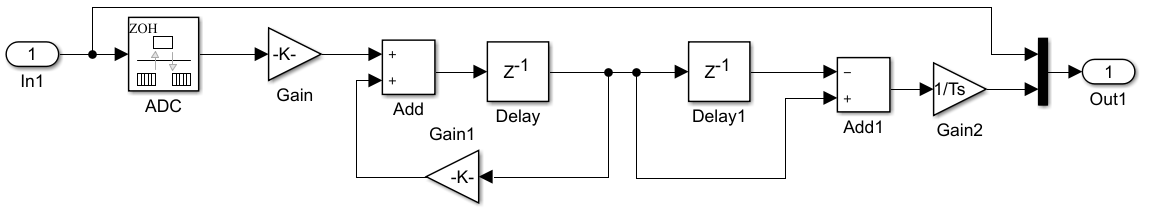
\includegraphics[width=\textwidth]{./part4_experiments/not_generated/simulink_estimator.png}
		\caption{estimator}
	\end{subfigure}
	\caption{simulink diagram}
	\label{fig:simulink measurement diagram}
\end{figure}

\subsection{Noise Analysis}
	$\theta$ and $\alpha$ have been measured before the low pass filter with no input signal, the signal measured is considered noise as displayed in figure~\ref{fig:time noise}. Instead of looking at the noise in function of time its very useful to look at the frequency spectrum and the histogram as is done in figure~\ref{fig:freq noise} and figure~\ref{fig:hist noise}. From the histogram we concluded that the noise is Gaussian. In the frequency spectrum you can see that there is a dominant low frequency band and a dominant frequency at 50Hz (net frequency). the rest of the spectrum is more or less flat so Gaussian noise is a good assumption.
	
	The variance of the noise can be computed and then used in the simulation. As the variance is the power in the signal $power = \frac{u_{eff}^2}{R} = \frac{stdev^2}{1 \Omega}$= variance
		
	\begin{figure}[H]
		\centering
		\begin{subfigure}[b]{0.30\textwidth}
			\includegraphics[width=\textwidth]{./part4_experiments/noise/simple_plot_2.png}
			\caption{timeplot of noise on $\theta$ and $\alpha$}
			\label{fig:time noise}
		\end{subfigure}
		\begin{subfigure}[b]{0.30\textwidth}
			\includegraphics[width=\textwidth]{./part4_experiments/noise/freq_spec.png}
			\caption{frequency spectrum noise $\theta$ $\alpha$}
			\label{fig:freq noise}
		\end{subfigure}
		\begin{subfigure}[b]{0.30\textwidth}
			\includegraphics[width=\textwidth]{./part4_experiments/noise/histogram_2.png}
			\caption{historgram of the noise}
			\label{fig:hist noise}
		\end{subfigure}
		\caption{noise measurement of $\theta$ and $\alpha$}
	\end{figure}


\subsection{step response}
	A step response of $-\frac{\pi}{4}$ is preformed in figure \ref{fig:step_1}. Compared to the step response in figure \ref{fig:simulation results noise} there's a continuous oscillation around the set-point. Both settling-times are similar, around 1 sec. There is a small steady state error that's probably due to the fact that the linearisation was made around $\theta = 0$. In figure \ref{driehoeksgolf} a triangle wave was given as reference input. There is some delay and the overshoot is due to the same problem as the steady state error, combined with the delay. 

	\begin{figure}[H]
		\centering
		\begin{subfigure}[b]{0.4\textwidth}
			\includegraphics[width=\textwidth]{./part4_experiments/tracking_manual/alpha_theta.png}
			\caption{states $\theta$ and $\alpha$}
		\end{subfigure}
		\begin{subfigure}[b]{0.4\textwidth}
			\includegraphics[width=\textwidth]{./part4_experiments/tracking_manual/alpha_theta_dot.png}
			\caption{states $\dot{\theta}$ and $\dot{\alpha}$}
		\end{subfigure}
		\begin{subfigure}[b]{0.4\textwidth}
			\includegraphics[width=\textwidth]{./part4_experiments/tracking_manual/motor_input.png}
			\caption{motor input}
		\end{subfigure}
		\caption{step response}
		\label{fig:step_1}
	\end{figure}
	
%\subsection{tracking}
%	\begin{figure}[H]
%		\centering
%		\begin{subfigure}[b]{0.45\textwidth}
%			\includegraphics[width=\textwidth]{./part4_experiments/tracking_sine/alpha_theta.png}
%			\caption{states $\theta$ and $\alpha$}
%		\end{subfigure}
%		\begin{subfigure}[b]{0.45\textwidth}
%			\includegraphics[width=\textwidth]{./part4_experiments/tracking_sine/alpha_theta_dot.png}
%			\caption{states $\dot{\theta}$ and $\dot{\alpha}$}
%		\end{subfigure}
%		\begin{subfigure}[b]{0.45\textwidth}
%			\includegraphics[width=\textwidth]{./part4_experiments/tracking_sine/motor_input.png}
%			\caption{motor input}
%		\end{subfigure}
%		\caption{tracking with a sine wave}
%	\end{figure}

	\begin{figure}[H]
		\centering
		\begin{subfigure}[b]{0.4\textwidth}
			\includegraphics[width=\textwidth]{./part4_experiments/tracking_stair/alpha_theta.png}
			\caption{states $\theta$ and $\alpha$}
		\end{subfigure}
		\begin{subfigure}[b]{0.4\textwidth}
			\includegraphics[width=\textwidth]{./part4_experiments/tracking_stair/alpha_theta_dot.png}
			\caption{states $\dot{\theta}$ and $\dot{\alpha}$}
		\end{subfigure}
		\begin{subfigure}[b]{0.4\textwidth}
			\includegraphics[width=\textwidth]{./part4_experiments/tracking_stair/motor_input.png}
			\caption{motor input}
		\end{subfigure}
		\caption{tracking with a triangular wave}
		\label{driehoeksgolf}
	\end{figure}
	
\newpage
\subsection{disturbances}
In figure \ref{dis_rej} you can see two disturbance rejection test, we think that the inverted pendulum is quite stable, because it reacts fast on the disturbance so is in less than 2 sec in its normal oscillating regime.

	\begin{figure}[H]
		\centering
		\begin{subfigure}[b]{0.45\textwidth}
			\includegraphics[width=\textwidth]{./part4_experiments/disturbance_rejection/alpha_theta.png}
			\caption{states $\theta$ and $\alpha$}
		\end{subfigure}
		\begin{subfigure}[b]{0.45\textwidth}
			\includegraphics[width=\textwidth]{./part4_experiments/disturbance_rejection/alpha_theta_dot.png}
			\caption{states $\dot{\theta}$ and $\dot{\alpha}$}
		\end{subfigure}
		\begin{subfigure}[b]{0.45\textwidth}
			\includegraphics[width=\textwidth]{./part4_experiments/disturbance_rejection/motor_input.png}
			\caption{motor input}
		\end{subfigure}
		\caption{disturbance rejection test}
		\label{dis_rej}
	\end{figure}
	

\subsection{The role of the cut-off frequency of the low pass filter}
When the cut-off frequency is to low, the inverted pendulum oscillates with a bigger amplitude, see figure~\ref{m_s_f}. Witch makes sense because the controller gets 'less' information and therefore can't react as fast.
But when the filter is set to high (above 3Hz) the controller react very heavy on the noise contained in the estimated states (see figure~\ref{e_s_f}). The motor starts to click a lot, see figure~\ref{m_o_f}. The ideal cut-off frequency is between 1-3 Hz. Therefore we keep 2 Hz for our experiments, because it is also a choice of what you prefer: a little bit faster reaction and a bit less amplitude in the oscillation or no clicking of the motor. It is clear that a cut-off frequency of above 3 Hz is highly unwanted for the equipment.

\begin{figure}[H]
	\centering
	\begin{subfigure}[b]{0.4\textwidth}
		\includegraphics[width=\textwidth]{./part5_experiments/FC05/alpha_theta.png}
		\caption{$f_c=0.5Hz$}
	\end{subfigure}
	\begin{subfigure}[b]{0.4\textwidth}
		\includegraphics[width=\textwidth]{./part5_experiments/FC1/alpha_theta.png}
		\caption{$f_c=1Hz$}
	\end{subfigure}
	\begin{subfigure}[b]{0.4\textwidth}
		\includegraphics[width=\textwidth]{./part5_experiments/FC2/alpha_theta.png}
		\caption{$f_c=2Hz$}
	\end{subfigure}
	\begin{subfigure}[b]{0.4\textwidth}
		\includegraphics[width=\textwidth]{./part5_experiments/FC3/alpha_theta.png}
		\caption{$f_c=3Hz$}
	\end{subfigure}
	\begin{subfigure}[b]{0.4\textwidth}
		\includegraphics[width=\textwidth]{./part5_experiments/FC4/alpha_theta.png}
		\caption{$f_c=4Hz$}
	\end{subfigure}
	\begin{subfigure}[b]{0.4\textwidth}
		\includegraphics[width=\textwidth]{./part5_experiments/FC8/alpha_theta.png}
		\caption{$f_c=4Hz$}
	\end{subfigure}
	\caption{measured $\theta$ and $\alpha$ states for different cut off frequencies}
	\label{m_s_f}
\end{figure}
\begin{figure}[H]
	\centering
	\begin{subfigure}[b]{0.4\textwidth}
		\includegraphics[width=\textwidth]{./part5_experiments/FC05/alpha_theta_dot.png}
		\caption{$f_c=0.5Hz$}
	\end{subfigure}
	\begin{subfigure}[b]{0.4\textwidth}
		\includegraphics[width=\textwidth]{./part5_experiments/FC1/alpha_theta_dot.png}
		\caption{$f_c=1Hz$}
	\end{subfigure}
	\begin{subfigure}[b]{0.4\textwidth}
		\includegraphics[width=\textwidth]{./part5_experiments/FC2/alpha_theta_dot.png}
		\caption{$f_c=2Hz$}
	\end{subfigure}
	\begin{subfigure}[b]{0.4\textwidth}
		\includegraphics[width=\textwidth]{./part5_experiments/FC3/alpha_theta_dot.png}
		\caption{$f_c=3Hz$}
	\end{subfigure}
	\begin{subfigure}[b]{0.4\textwidth}
		\includegraphics[width=\textwidth]{./part5_experiments/FC4/alpha_theta_dot.png}
		\caption{$f_c=4Hz$}
	\end{subfigure}
	\begin{subfigure}[b]{0.4\textwidth}
		\includegraphics[width=\textwidth]{./part5_experiments/FC8/alpha_theta_dot.png}
		\caption{$f_c=4Hz$}
	\end{subfigure}
	\caption{calculated $\dot{\theta}$ and $\dot{\alpha}$ states for different cut off frequencies}
	\label{e_s_f}
\end{figure}

\begin{figure}[H]
	\centering
	\begin{subfigure}[b]{0.4\textwidth}
		\includegraphics[width=\textwidth]{./part5_experiments/FC05/motor_input.png}
		\caption{$f_c=0.5Hz$}
	\end{subfigure}
	\begin{subfigure}[b]{0.4\textwidth}
		\includegraphics[width=\textwidth]{./part5_experiments/FC1/motor_input.png}
		\caption{$f_c=1Hz$}
	\end{subfigure}
	\begin{subfigure}[b]{0.4\textwidth}
		\includegraphics[width=\textwidth]{./part5_experiments/FC2/motor_input.png}
		\caption{$f_c=2Hz$}
	\end{subfigure}
	\begin{subfigure}[b]{0.4\textwidth}
		\includegraphics[width=\textwidth]{./part5_experiments/FC3/motor_input.png}
		\caption{$f_c=3Hz$}
	\end{subfigure}
	\begin{subfigure}[b]{0.4\textwidth}
		\includegraphics[width=\textwidth]{./part5_experiments/FC4/motor_input.png}
		\caption{$f_c=4Hz$}
	\end{subfigure}
	\begin{subfigure}[b]{0.4\textwidth}
		\includegraphics[width=\textwidth]{./part5_experiments/FC8/motor_input.png}
		\caption{$f_c=8Hz$}
	\end{subfigure}
	\caption{motor input for different cut off frequencies}
	\label{m_o_f}
\end{figure}


